\vspace{-3cm}\chapter{实验2. 数字转英语}

\section{2.1 题目}

编写一个程序,从\textbf{命令行参数}中读取一个范围为[-999999999,  999999999]的整数,
输出为这个整数转换成英语表示的等价形式。下面列出程序中可能需要用到的所有数
字表示的英文单词:negative, zero, one, two, three, four, five, six, seven, eight, nine, ten, 
eleven,twelve,  thirteen,  fourteen,  fifteen,  sixteen,  seventeen,  eighteen,  nineteen,  twenty,  
thirty,forty, fifty, sixty, seventy, eighty, ninety, hundred, thousand, million。

注意:在转换过程中,尽可能使用\textbf{更大的数字单位}。比如1500 这个数字应该的表示为one thousand 
five hundred,而不应该是 fifteen hundred。

举例: 
数字 123419 转换成的英语表示为: 
one hundred twenty three thousand four hundred nineteen.

\section{2.2 题目分析}

\begin{enumerate}
    \item \textbf{数据输入}. 注意到本题的输入范围在Java的\lstinline{int}范围内,所以可以通过\lstinline{Integer.parseInt}直接得到数字。
    \item \textbf{数据处理}. 
    \begin{itemize}
        \item 可以参照英语的用语习惯,每三位划分,由数据范围可知最多划分成高中低三部分,分别用million和thousand分开,每一部分
            的打印逻辑都相同,可以总结为一个\lstinline{void print_3digit(int a)}函数。
        \item 为了避免负数可能导致的取余等计算问题,判断输入为负数并打印negative后即可。如果输入为0直接打印zero结束运行即可。
        \item 特殊:如果输入为0直接打印zero结束运行即可
    \end{itemize}
    \item 
\end{enumerate}

\section{2.3 代码展示}

代码和注释如下所示,核心函数为\lstinline{void print_3digit(int a)}(line26),该函数将输入的三位数打印出来,这一过程又分为打印hundred
和两位数打印\lstinline{void print_2digit(int a)}(line35).
\lstinputlisting[
    language = Java, 
    caption = {\bf Problem2.java}
]{../../../ProblemSet/src/Problem2.java}

\section{2.4 结果展示}

\begin{figure}[H]
	\centering
	\begin{subfigure}{0.13\linewidth}
		\centering
		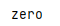
\includegraphics[width=0.5\linewidth]{../pic/2/2.1.png}
        \caption{input: 0}
	\end{subfigure}
	\begin{subfigure}{0.17\linewidth}
		\centering
		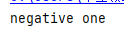
\includegraphics[width=1\linewidth]{../pic/2/2.2.png}
        \caption{input: -1}
	\end{subfigure}
	\begin{subfigure}{0.17\linewidth}
		\centering
		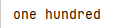
\includegraphics[width=1\linewidth]{../pic/2/2.3.png}
        \caption{input: 100}
	\end{subfigure}
    \begin{subfigure}{0.17\linewidth}
		\centering
		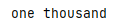
\includegraphics[width = 1\linewidth]{../pic/2/2.4.png}
        \caption{input: 1000}
	\end{subfigure}
	\begin{subfigure}{0.27\linewidth}
		\centering
		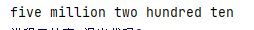
\includegraphics[width=1\linewidth]{../pic/2/2.5.png}
        \caption{input: 5000210}
	\end{subfigure}
	\begin{subfigure}{1\linewidth}
		\centering
		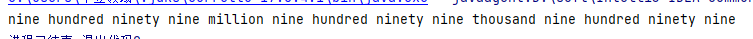
\includegraphics[width=0.9\linewidth]{../pic/2/2.6.png}
        \caption{input: 999999999}
	\end{subfigure}
	\caption{Output of Problem2}
\end{figure}

\section{2.5 总结与收获}

\begin{itemize}
    \item 程序一开始的设计过程并没有题目分析中写的那么有条理,函数的需要是在程序编写过程中感觉到的;
    \item idea自动把\lstinline{switch}的默认语法转换成一种更短更新颖易读的写法,之前从没接触过;
    \item \textbf{空格处理.} 我们已经将输出模块化了,虽然题目中没有要求,但如何在单词之间设计优雅的空格是一个值得思考的问题,
        具体设计过程会涉及很多条件处理。
\end{itemize}